\documentclass[11pt]{article}

\usepackage[review]{acl}
\usepackage{times}
\usepackage{latexsym}
\usepackage{amsmath,amssymb}
\usepackage{booktabs}
\usepackage{graphicx}
\usepackage{microtype}
\usepackage{xcolor}
\usepackage{multirow}
\usepackage{url}

\graphicspath{{../figures/}}

\newcommand{\rpi}{R_{\mathrm{PI}}}
\newcommand{\dinert}{D_{\mathrm{inert}}}
\newcommand{\iflip}{I_{\mathrm{flip}}}
\newcommand{\fshared}{F_{\mathrm{shared}}}
\newcommand{\yes}{\textsc{yes}}
\newcommand{\no}{\textsc{no}}

\title{When Consensus Lies: Intervention-Tested Provenance for Reliable Multi-Agent LLM Decisions}

\author{Anonymous ACL submission}

\begin{document}
\maketitle

\begin{abstract}
Agreement among language-model agents is often treated as independent corroboration even when agents share a model, prompts, or evidence roots. This creates \emph{false consensus}: a highly agreed answer can be wrong because agents repeat the same unsupported or behaviorally irrelevant evidence. We ask two linked questions: can observable evidence dependence identify wrong consensus before labels are revealed, and when is that reliability information strong enough to route a decision rather than retain the consensus? We formulate and preregister an environment-controlled protocol that records source-to-evidence provenance and applies paired removal, reversal, and substitution interventions without inspecting hidden chain-of-thought. A frozen outcome-independent score, $\rpi$, combines intervention inertia, answer-flip inertia, and citation overlap.

We evaluate five Qwen3.5-4B agents on provenance-disjoint BoolQ splits. A first 200-question held-out run was directionally positive but inconclusive (AUROC 0.605, 95\% CI [0.495, 0.721]). A preregistered replication used every remaining eligible validation root: 358 questions and 7,160 calls. Among 300 high-consensus questions, 66 were wrong. $\rpi$ ranked wrong consensus with AUROC 0.705 [0.620, 0.781] and reduced retained error at 80\% coverage from 0.220 to 0.133 (reduction 0.087 [0.046, 0.098]). BoolQ label subgroups reverse direction, and citation overlap alone is at chance.

A preregistered label-symmetric cross-family test then uses 250 natural contrastive Wikipedia pairs from VitaminC (500 balanced items; 10,000 calls per model) with Qwen3.5-4B and Ling-3.0-tiny. The separately frozen V3.16 score reaches AUROC 0.808 [0.761, 0.853] for Qwen and 0.761 [0.722, 0.798] for Ling, with Risk@80 error reductions of 0.048 and 0.041. All performance intervals clear their registered thresholds, but the joint pass is withheld because Ling has 17 high-consensus SUPPORTS errors versus the preregistered minimum of 20. This is bounded per-model cross-family evidence, not a universal transfer claim.

We also evaluate an as-of-provenance S\&P~500 replay. Five LLM agents answer 5-day-ahead direction questions on 500 dates across two paired protocol versions. The router attains the best calibration but no confirmatory AURC advantage; the V1$\to$V2 pair exposes a preregistered prompt-only repair for fail-closed output failures. Intervention-tested provenance is thus a falsifiable reliability signal---not consensus, confidence, financial alpha, or universal robustness.
\end{abstract}

\section{Introduction}

Multi-agent language-model systems commonly sample several agents, assign roles, and aggregate their votes. Debate and collaboration can improve reasoning and factuality \citep{du2023multiagent,liang2023divergent}, but a majority is informative only to the extent that its information and errors are sufficiently diverse. Five agreeing agents are not five independent witnesses when they inherit the same model bias or cite overlapping evidence. Empirical conformity effects reinforce this concern \citep{choi2025conformity}.

We study \emph{high-consensus answers supported by correlated evidence}. An answer is a harmful false consensus when at least 80\% of agents agree and their consensus is wrong. Confidence and vote agreement describe the answer as produced, but not whether the decision responds appropriately when its claimed evidence changes. Citation correctness is likewise insufficient: agents may cite relevant text after committing to an answer, and apparently distinct passages may descend from one provenance root.

Our evaluation environment, rather than the language model, therefore controls evidence identity and interventions. Each agent receives a fixed subset of evidence IDs and returns only a binary answer, confidence, and cited IDs. For the same question--agent pair, the environment removes evidence, reverses its direction, or substitutes an opposite-answer passage. We observe answer changes and citation overlap without collecting private reasoning traces. Figure~\ref{fig:framework} summarizes the resulting decision pipeline.

We deliberately do not claim that input intervention, evidence binding, selective prediction, or multi-agent conformity is individually new. Prior work has studied semantic faithfulness under deletion and negation, explanation faithfulness under contradiction, mechanized evidence contracts, and debate selection based on confidence or disagreement \citep{chaturvedi-etal-2024-analyzing,chuang-etal-2026-faithlm,xu-etal-2026-gavel,verma-etal-2026-selene}. Our distinct object is the pre-outcome error risk of a fixed multi-agent consensus under environment-assigned evidence conditions: evidence identity is external to the model, the same agent view is paired across conditions, and the result is evaluated against a subsequently revealed consensus error rather than explanation quality, citation sufficiency, or debate accuracy.

\begin{figure*}[t]
    \centering
    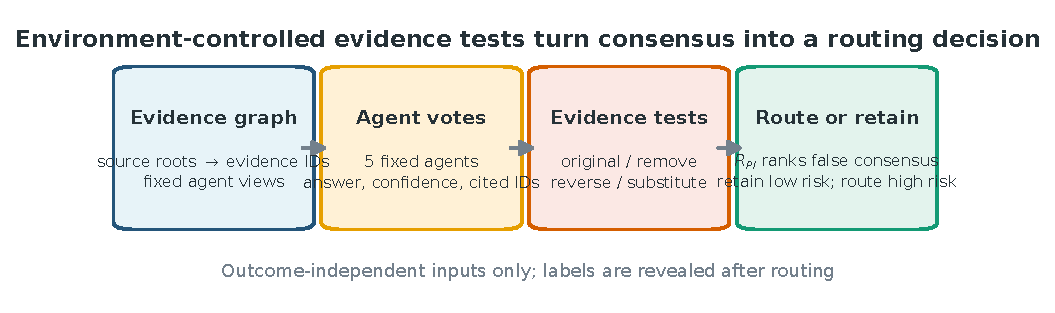
\includegraphics[width=\textwidth]{framework_overview.pdf}
    \caption{The environment maintains provenance, assigns fixed evidence views, and applies paired interventions. Only outcome-independent behavior and citation structure enter the registered risk score ($\rpi$ or $R_{\mathrm{sym}}$). The router retains lower-risk consensus and defers higher-risk decisions; labels are revealed only for evaluation.}
    \label{fig:framework}
\end{figure*}

The paper separates two questions that are often conflated. \textbf{Reliability ranking} asks whether an intervention-based score ranks wrong consensus above correct consensus. \textbf{Routing sufficiency} asks whether that ordering is useful at a frozen operating point. A positive AUROC alone does not license a router: at the selected coverage, retained error must improve on unseen questions, and uncertainty may still make that improvement inconclusive. Conversely, when evidence is insufficient, retaining the consensus is preferable to inventing a post-hoc threshold.

Our experiments follow a versioned sequence. A development run exposed an outcome-leaking metric; we invalidate it despite its favorable score. A first untouched BoolQ validation was underpowered under its registered confidence-interval rule. A larger provenance-disjoint replication then passed the unchanged primary endpoint, while a label-symmetric cross-family protocol produced strong per-model evidence but failed one preregistered adequacy gate. A sequential market replay then failed its routing endpoint while exposing an output-contract failure. We preserve all stages because negative and invalidated results are part of the method's validity evidence.

Our contributions are:

\begin{itemize}
    \item A pre-outcome consensus-error audit that specifies an environment-maintained evidence graph, fixed agent views, paired removal, reversal, and substitution conditions, and observable decision outcomes. The individual intervention and citation ingredients are established tools; the contribution is their use in this consensus-error estimand with an explicit integrity protocol.
    \item Versioned pre-outcome risk contracts: $\rpi$ for the original BoolQ study and $R_{\mathrm{sym}}$ for the label-symmetric V3.16 transfer, both with explicit outcome firewalls.
    \item A preregistered real-LLM BoolQ replication and a label-symmetric cross-family stress test, with label-conditional and event-count boundaries preserved rather than repaired post hoc.
    \item A decision-centered external stress program: S\&P~500 replays separate risk ranking, calibration, and output-contract validity, and report no confirmatory routing gain.
    \item A preregistered protocol-failure chain with paired prompt repair and preserved induced failure modes.
\end{itemize}

\section{False Consensus under Evidence Dependence}

\subsection{Decisions and environment-held provenance}

For question $q$, let $E_q=\{e_1,e_2,e_3\}$ denote evidence units with environment-assigned IDs and source roots. Agent $i$ receives a fixed view $V_{qi}\subset E_q$ and returns
\begin{equation}
o_{qi}=(a_{qi},c_{qi},C_{qi}),
\end{equation}
where $a_{qi}\in\{0,1\}$ is the answer, $c_{qi}\in[0,1]$ is confidence, and $C_{qi}\subseteq V_{qi}$ contains cited evidence IDs. Citations outside the assigned view are rejected. We use five fixed agents.

The original-condition consensus is $\hat y_q=\operatorname{majority}_i a_{qi}^{(0)}$, with agreement $A_q$ equal to the fraction selecting $\hat y_q$. The high-consensus subset is fixed as $A_q\geq0.8$. Only after routing do we reveal the native label $y_q$ and compute
\begin{equation}
z_q=\mathbb{1}[\hat y_q\neq y_q].
\end{equation}
The primary task is to rank $z_q=1$ above $z_q=0$ within the high-consensus subset using pre-outcome observations only.

Agreement can reflect independent evidence, shared valid evidence, or a common failure. Vote counts cannot distinguish these cases. We therefore retain the graph
\begin{equation}
\begin{aligned}
\text{source root}&\rightarrow\text{evidence ID}\rightarrow\text{agent view}\\
&\rightarrow\text{citation}\rightarrow\text{answer}.
\end{aligned}
\end{equation}
Two agents citing evidence from one root do not become two independent sources.

\subsection{Paired evidence interventions}

Each original response is paired with three conditions:
\begin{itemize}
    \item \textbf{remove}: delete an assigned evidence unit;
    \item \textbf{reverse}: replace its directional content with an opposite-answer form;
    \item \textbf{substitute}: insert a separately generated opposite-answer sentence constrained to the original topic, entities, and length window.
\end{itemize}
The model, persona, output schema, and evidence partition remain fixed. These tests ask an operational faithfulness question: does the observable decision depend on the evidence it was instructed to use? This complements factuality and attribution benchmarks \citep{thorne2018fever,lin2022truthfulqa,muller2023attribution} and follows the broader distinction between plausible explanations and faithful dependence \citep{jacovi2020faithfully,wiegreffe2019attention}.

These are operational response tests, not causal identification of the model's internal evidence use. Invariance can reflect robust inference, evidence irrelevance, or failure to process the intervention; a changed answer can reflect an artifact of the transformed text. The endpoint therefore tests predictive utility for later consensus error, not semantic entailment or internal causal faithfulness.

\section{Intervention-Tested Reliability}

\subsection{Observable risk coordinates}

For each question we compute three quantities in $[0,1]$:
\begin{enumerate}
    \item \textbf{Complete intervention inertia} $\dinert$: the fraction of agents whose answer never changes under removal, reversal, or substitution.
    \item \textbf{Flip inertia} $\iflip$: one minus the mean answer-flip rate over all $5\times3$ agent--intervention pairs.
    \item \textbf{Shared-source fraction} $\fshared$: the fraction of agents whose original citations overlap a previously observed agent under a fixed ordering.
\end{enumerate}
High values indicate risk: a team that remains unchanged when evidence is removed or contradicted is behaviorally suspicious, while shared citations lower the effective independence of agreement.

\subsection{Frozen score and leakage barrier}

One development split selected among 66 convex combinations on a 0.1-spaced simplex. The following score was frozen before either validation experiment:
\begin{equation}
\begin{aligned}
\rpi(q)={}&0.1\dinert(q)+0.3\iflip(q)\\
&+0.6\fshared(q).
\end{aligned}
\label{eq:rpi}
\end{equation}
The implementation accepts only these three fields. Labels, correctness, harmful-consensus indicators, and aliases are forbidden. A regression test poisons every outcome field while holding the allowlisted inputs fixed and requires the score to remain identical.

We use $\rpi$ for this original BoolQ contract only. V3.16 freezes a separate label-symmetric instantiation of the same intervention-tested risk family:
\begin{equation}
R_{\mathrm{sym}}(q)=0.3\,D_{\mathrm{rev}}(q)+0.7\,D_{\mathrm{int}}(q),
\label{eq:rsym}
\end{equation}
where $D_{\mathrm{rev}}$ is reverse inertia and $D_{\mathrm{int}}$ is intervention disagreement. $R_{\mathrm{sym}}$ was selected with pair-grouped nested out-of-fold development data before formal Qwen and Ling outcomes were accessed. The two scores share the outcome firewall and error-ranking notation, but their formal results are not pooled and neither score is retuned after formal outcome access.

\subsection{Route or retain}

At coverage $\kappa=0.8$, the selective router sorts high-consensus questions by increasing $\rpi$ and retains the lowest-risk 80\%. Remaining questions are routed to a fallback; the method does not change or repair their answers. We report baseline error, retained error, absolute reduction, and a question-bootstrap interval. This is selective prediction \citep{geifman2017selective}: lower retained risk is purchased by deferral.

Our interpretation has two levels. The preregistered primary endpoint evaluates risk ordering with AUROC. The frozen routing point is secondary and evaluates decision utility. We do not search the coverage curve for a favorable point after observing labels. Other coverages are shown only to reveal the behavior of the score, not to replace the 80\% result.

\section{Experimental Setup}

\subsection{BoolQ and evidence construction}

BoolQ contains naturally occurring yes/no questions paired with Wikipedia passages \citep{clark2019boolq}. We use the official training split only for development and the validation split for V11.1 and V12.1. A frozen text-only rule extracts three 8--80-token sentences whose TF--IDF similarity lies inside an evidence-diversity band. V11.1 selects 100 \yes{} and 100 \no{} roots by salted hashing. V12.1 uses all 358 remaining eligible validation roots (246 \yes{}, 112 \no{}), with zero source-root overlap.

An earlier FEVER audit found that 1,602 of 1,766 candidate triples (90.7\%) exceeded the maximum evidence-overlap threshold; only 29 (1.6\%) survived the full band. The formal run therefore stopped before any LLM call. We treat this as a dataset boundary: redundant evidence clusters cannot test independent corroboration merely by assigning different personas.

\textbf{VitaminC label-symmetric transfer.} The real VitaminC archive contains natural SUPPORTS/REFUTES pairs sharing a claim and page root. A strict character-similarity and token-overlap filter retained 573 usable page roots; the frozen split used 4 smoke pairs, 30 development pairs, and 250 formal pairs. Each formal pair contributes one SUPPORTS and one REFUTES item, yielding 500 exactly balanced items with globally disjoint target and distractor roots. The dataset labels are used only to construct and audit this balanced design; they are withheld from model calls, risk computation, route selection, and the evaluator until the pre-outcome artifacts are frozen.

\subsection{Model and agents}

All language-model calls use locally deployed instruction models through OpenAI-compatible endpoints: Qwen3.5-4B (BoolQ and V3.16), Ling-3.0-tiny (V3.15.2 and V3.16), and Hy-MT2-7B (LLM-S\&P500 V1/V2). The five fixed personas are a literal evidence user, skeptical auditor, consistency checker, counterfactual reasoner, and minimal judge. V3.16 uses five personas, four conditions per item, a prompt-only JSON interface, a strict local parser, a 256-token cap, fixed model-specific seeds, and fresh model-specific formal caches. BoolQ V11.1/V12.1 achieved 100\% schema validity and 100\% first-pass validity. Four concurrent clients produced V12.1; server-side GPU allocation was unobservable, so we make no four-GPU execution claim.

\subsection{Frozen protocol sequence}

Appendix Table~\ref{tab:protocols} separates development, auxiliary aborts, validation, cross-family transfer, and replay generations. V11.1 and V12.1 amendments were frozen after observing only auxiliary rewrite-format failures and before any validation-agent outcome. V3.16 was frozen after Qwen development and Ling transport qualification but before either model's 500-item formal outcomes. The replay V2 manifest is sha-pinned to V1, making the comparison date-paired.

\subsection{Metrics and uncertainty}

The BoolQ primary endpoint is
\begin{equation}
\operatorname{AUROC}(\rpi,z\mid A\geq0.8).
\end{equation}
The BoolQ pass rule requires at least 80 high-consensus questions, at least ten cases per class, and a 1,000-replicate question-bootstrap 95\% CI lower bound strictly above 0.5. Secondary metrics include AUPRC, individual coordinates, all-question harmful-consensus ranking, intervention flip rates, and error at 80\% coverage. Native-label subgroups and pooled V11.1+V12.1 analyses were preregistered as descriptive and cannot replace the aggregate primary endpoint.

V3.16 uses $R_{\mathrm{sym}}$ on the same pre-outcome error-ranking target with pair-bootstrap intervals. Each model must pass transport validity, at least 400 high-consensus items, at least 20 high-consensus errors in each native label, overall/macro/worst-label AUROC lower bounds above 0.5, and a positive Risk@80 error-reduction interval. The cross-family headline requires both models to pass every gate; pooled data cannot rescue a failed model or label.

\section{Results}

\subsection{Can interventions identify false consensus?}

The first held-out evaluation contained 180 high-consensus questions and 30 errors. Its AUROC was 0.605 [0.495, 0.721], directionally consistent but inconclusive under the frozen rule. V12.1 contained 300 high-consensus questions and 66 errors. Without changing the score or endpoint, $\rpi$ achieved AUROC 0.705 [0.620, 0.781] and AUPRC 0.414. The lower confidence bound clears chance. The descriptive pooled AUROC over 480 high-consensus questions is 0.669 [0.602, 0.738]. Figure~\ref{fig:primary}a shows all three estimates.

\begin{figure*}[t]
    \centering
    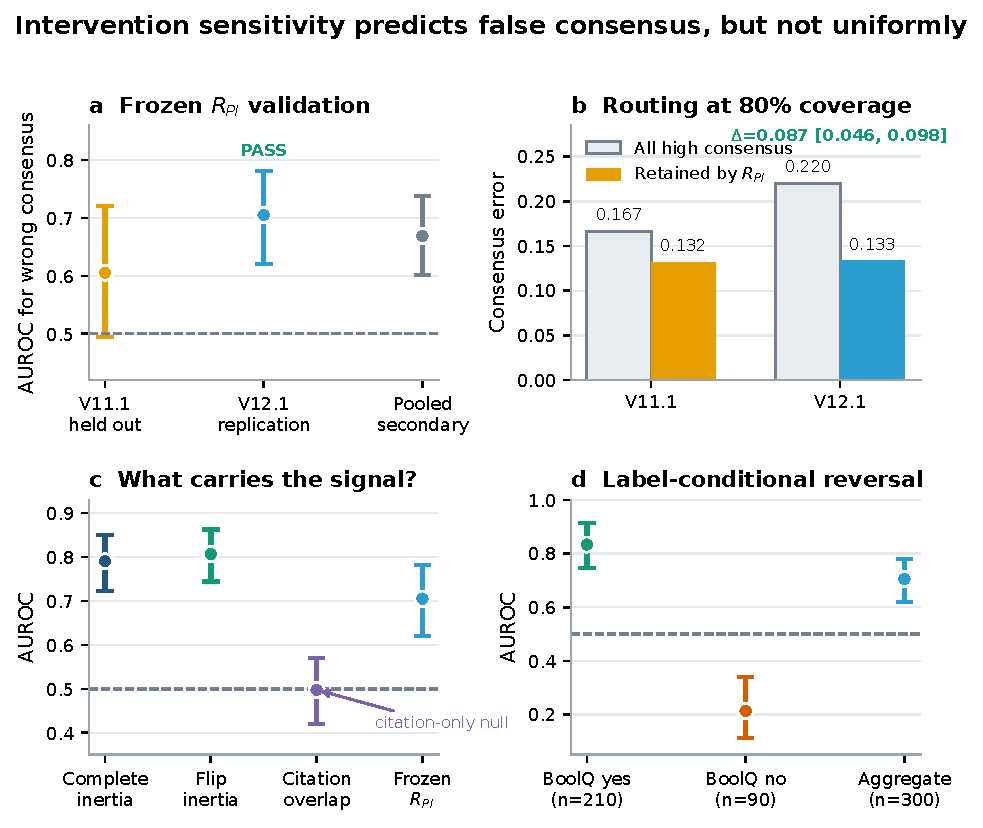
\includegraphics[width=\textwidth]{primary_results.pdf}
    \caption{Main BoolQ findings. (a) The frozen score is inconclusive in V11.1 and passes the registered AUROC rule in V12.1; pooling is secondary. (b) At 80\% coverage, V12.1 retained error falls from 0.220 to 0.133. (c) Behavioral intervention coordinates carry the signal, whereas citation overlap alone is near chance. (d) Opposite label-conditional directions limit the aggregate claim. Error bars are question-bootstrap 95\% intervals.}
    \label{fig:primary}
\end{figure*}

\subsection{When does reliability support routing?}

At the frozen 80\% coverage point, V12.1 retained the 240 lowest-risk high-consensus questions. Error fell from 0.220 to 0.133, an absolute reduction of 0.087 [0.046, 0.098]. In V11.1, error fell from 0.167 to 0.132, but the smaller reduction of 0.035 had interval [0.000, 0.069]. Thus the first run suggested useful ordering without establishing operating-point benefit; the larger disjoint replication supplies the stronger routing evidence.

This distinction answers the paper's decision question. Consensus is retained for the lower-risk region and routed only at the frozen risk rank. When the held-out interval includes no improvement, as in V11.1, reliability information is insufficient for a strong routing claim. We do not tune a V11.1 threshold or discard the run. Figure~\ref{fig:primary}b shows the registered comparison; the full descriptive curve appears in Appendix Figure~\ref{fig:routing}.

\subsection{What information carries the signal?}

On V12.1, complete intervention inertia achieves AUROC 0.791 [0.724, 0.850], and flip inertia achieves 0.807 [0.744, 0.863]. Shared-source fraction alone is 0.498 [0.419, 0.571]. Removal, reversal, and substitution answer-flip rates are 0.470, 0.327, and 0.301, respectively.

The result narrows the mechanism claim. Provenance is useful when it defines controlled manipulations and dependence structure; counting shared citations is not sufficient. The frozen formula places 0.6 weight on the null coordinate, so a new score might improve, but retuning on V12.1 would invalidate the replication and is not performed.

\subsection{Label-conditional reversal}

The preregistered descriptive subgroups expose a major limitation. Among 210 high-consensus native-\yes{} questions, AUROC is 0.834 [0.747, 0.913]. Among 90 native-\no{} questions, AUROC is 0.213 [0.112, 0.339]. The aggregate pass is therefore not label invariant. Possible mechanisms include asymmetric evidence construction, response priors, and intervention polarity, but V12.1 was not designed to distinguish them. We perform no corrective subgroup reweighting after observing the result.

The follow-up makes this limitation explicit rather than treating it as a footnote. V3.15.2 applied the frozen BoolQ protocol to Ling-3.0-tiny and reproduced the aggregate endpoint, but its label AUROC was 0.957 for \yes{} and 0.120 for \no{}. We therefore did not call it label-robust. V3.16 instead uses balanced natural contrastive pairs and evaluates native labels separately.

\subsection{Label-symmetric cross-family transfer (VitaminC V3.16)}

V3.16 freezes 250 natural contrastive Wikipedia pairs from VitaminC: each pair contributes one SUPPORTS and one REFUTES item, with globally disjoint target and distractor roots. Each of five agents receives the original, remove, reverse, and substitute conditions, for 10,000 calls per model. The dataset labels are used for pair construction and balance auditing only, and are withheld from model calls, risk computation, route selection, and the evaluator until pre-outcome artifacts are frozen. The separate $R_{\mathrm{sym}}$ score is selected on Qwen development data and then held fixed for Qwen and Ling formal evaluation. This is directional Qwen-development-to-Qwen/Ling transfer, not bidirectional model generalization.

\begin{table}[t]
\centering
\small
\setlength{\tabcolsep}{2.5pt}
\begin{tabular}{lrrrrrr}
\toprule
Model & $N_{\mathrm{hc}}$ & Err. & AUROC & Macro & Worst & Risk@80 \\
\midrule
Qwen & 482 & 87 & 0.808 & 0.811 & 0.792 & .180$\to$.132 \\
Ling & 464 & 113 & 0.761 & 0.766 & 0.635 & .244$\to$.202 \\
\bottomrule
\end{tabular}
\caption{V3.16 label-symmetric transfer. Qwen's overall AUROC CI is [0.761, 0.853] and Ling's is [0.722, 0.798]. The joint gate fails only on Ling's native-label event count, not on the reported performance intervals.}
\label{tab:v316}
\end{table}

Qwen's pair-bootstrap intervals are [0.761, 0.853] for overall AUROC, [0.763, 0.856] for macro AUROC, [0.729, 0.844] for worst-label AUROC, and [+0.025, +0.067] for Risk@80 error reduction. Ling's corresponding intervals are [0.722, 0.798], [0.719, 0.816], [0.546, 0.732], and [+0.026, +0.058]. The four model-label AUROCs all exceed 0.63. However, Ling has only 17 high-consensus SUPPORTS errors (versus 96 REFUTES errors), below the frozen minimum of 20, so the preregistered joint PASS is withheld. This is an adequacy failure, not a reason to pool selected errors or add post-hoc examples.

The formal primary remains the frozen $R_{\mathrm{sym}}$ composite. Reverse inertia alone is descriptively stronger (AUROC 0.855 for Qwen and 0.837 for Ling), while intervention disagreement alone is weak; neither observation changes the registered score. At identical high-consensus counts, $R_{\mathrm{sym}}$ also exceeds confidence and vote-disagreement AUROC: Qwen 0.808 versus 0.601 and 0.512, and Ling 0.761 versus 0.568 and 0.522. Risk ranks correlate only 0.295 between models on 449 common high-consensus items, so the result supports aggregate mechanism transfer rather than stable item-level ranking or universal robustness.

\section{Validity Audits and External Stress Test}

\paragraph{Outcome leakage.}
V10.4 originally emitted a positive-looking \texttt{shared\_weighted} AUROC of 0.959. A post-run audit found that the metric multiplied citation overlap by a term containing answer correctness. It is invalid for pre-outcome routing. We preserve the records, invalidate the verdict, and use the failure to motivate the explicit allowlist in Eq.~\ref{eq:rpi}.

\paragraph{Auxiliary aborts.}
V10.1--V10.3, V11, and V12 stopped under registered rewrite-quality gates before evaluation outcomes existed. No later-ranked question replaced a failed item. These runs are instrumentation evidence, not router results.

\paragraph{Sequential cross-domain stress test.}
We additionally mapped the intervention framework to an as-of S\&P~500 replay. Statistical-agent V4/V5 replays show favorable operating points but a preregistered AURC difference of $-0.0078$ with interval $[-0.0607,0.0459]$. The LLM V1/V2 replay uses five roles on 500 dates (2,500 calls per version) and an identical manifest. Its router has the best V1 risk ECE (0.055 versus 0.174 for majority), but the AURC difference is $-0.0874$ [\(-0.1994,0.0736\)] in V1 and $+0.0317$ [\(-0.0886,0.1805\)] in V2. The paired prompt-only repair raises valid responses from 68.2\% to 75.6\%, while the routing endpoint remains non-confirmatory. This is an external-validity and protocol boundary, not evidence of financial alpha or general cross-domain transfer. Full details are in Appendix~\ref{sec:finance}.

\section{Related Work}

\paragraph{Multi-agent reasoning.}
Multi-agent debate elicits proposals and revisions from several model instances \citep{du2023multiagent,liang2023divergent}, while conformity work shows that group interaction can amplify dominant stances \citep{choi2025conformity}. We study a different unit: whether an already formed agreement is trustworthy when its evidence and errors are dependent.

\paragraph{Closest neighboring protocols.}
Input-intervention work tests semantic effects on a single model's QA inference \citep{chaturvedi-etal-2024-analyzing}; FaithLM measures and optimizes explanation faithfulness under contradiction \citep{chuang-etal-2026-faithlm}. GAVEL binds atomic subclaims to evidence and mechanizes citation scrutiny \citep{xu-etal-2026-gavel}, while SELENE uses confidence and disagreement to initiate debate \citep{verma-etal-2026-selene}. We do not claim these ingredients are new: our unit is a fixed multi-agent consensus, whose environment-held evidence conditions are tested for predicting an unrevealed consensus error.

\paragraph{Truthfulness, attribution, and faithfulness.}
TruthfulQA, FEVER, and attribution work provide task and evidence-quality contexts \citep{lin2022truthfulqa,thorne2018fever,muller2023attribution}. Faithfulness work distinguishes plausible explanations from dependence \citep{jacovi2020faithfully,wiegreffe2019attention}; our endpoint is pre-outcome error ranking of a consensus, not explanation quality or citation sufficiency.

\paragraph{Selective prediction and uncertainty.}
Selective classification and calibration quantify abstention risk and probability quality \citep{geifman2017selective,guo2017calibration}; conformal methods provide guarantees under stated assumptions \citep{angelopoulos2021conformal}. We use empirical risk--coverage and bootstrap uncertainty; these tools evaluate, but do not define, our evidence-response estimand.

\section{Conclusion}

Consensus is informative only to the extent that its evidence and errors are sufficiently independent. We formulate an environment-controlled framework that turns provenance into paired behavioral tests and a selective risk signal. A provenance-disjoint BoolQ replication confirms error ranking at fixed 80\% coverage; a label-symmetric VitaminC transfer yields strong per-model evidence on Qwen and Ling while withholding the joint pass for a frozen event-count gate. The sequential replay locates a second boundary: calibration and protocol diagnosis transfer, but confirmatory routing gain does not yet.

The resulting principle is decision-centered: retain consensus when intervention evidence indicates lower risk, route the higher-risk tail only at a frozen operating point, and withhold a routing claim when uncertainty includes no benefit. A fresh-root V3.16 replication sized before outcome access is the next empirical step; it must preserve $R_{\mathrm{sym}}$ and cannot pool selected formal errors.

\section*{Limitations}

Completed language-model experiments use Qwen3.5-4B, Ling-3.0-tiny, and Hy-MT2-7B; the five personas within each deployment are not independent models. V3.16 provides cross-family evidence on one balanced VitaminC setting, but its joint adequacy gate is withheld because Ling has fewer than 20 SUPPORTS errors, and item-level risk Spearman is only 0.295. The LLM replay has wide intervals at 150 test dates and no stronger-model replication.

V12.1 label subgroups reverse direction, and V3.15.2 reproduces this pattern on Ling. V3.16 reduces the asymmetry with balanced natural pairs but cannot identify whether the remaining difference comes from answer priors, evidence construction, or intervention polarity. We therefore make no arbitrary-QA or universal-factuality claim.

$\rpi$ was selected on one 100-question development split, while $R_{\mathrm{sym}}$ was selected on Qwen V3.16 development data. Reverse inertia is stronger descriptively, but replacing either frozen score after formal outcomes would be post-hoc.

Generated substitutes may differ in fluency or logical force; the interventions measure different response behaviors and do not identify one unique causal mechanism. Abstention defers rather than solves risky questions.

The paper is a detection study rather than a universal answer-repair study; recovery experiments remain supplementary and do not convert V3.16 into a repair claim.

Finally, the financial replay is retrospective and uses a locally substituted 7B backend under a registered deviation. Its primary AURC intervals cross zero; it cannot establish prospective performance, alpha, or causal market impact.

The submission still needs final literature, license, compute, and V3.16 error-example audits, plus a supplement separating answer repair from detection.

\section*{Ethical Considerations}

False consensus matters in medicine, law, finance, and content moderation. A provenance-aware signal may help identify when many agreeing agents repeat one weak source, but it can also create false reassurance. Low $\rpi$ is not proof of correctness, and an intervention-sensitive answer can remain wrong. We recommend using routing for triage and independent evidence acquisition, not as an autonomous truth certificate.

The experiments use existing QA datasets and automated model outputs. We collect no private human data or hidden chain-of-thought. Financial results are research diagnostics and should not be interpreted as investment advice.

\bibliography{references}

\appendix

\section{Frozen Risk Contract}

\begin{verbatim}
Allowed:   D_inert, flip_inertia, frac_shared
Forbidden: label, gold_binary, correct,
           any_wrong, harmful_fc, aliases

R_PI = 0.1 * D_inert
     + 0.3 * flip_inertia
     + 0.6 * frac_shared

Primary subset: original agreement >= 0.8
Primary: AUROC(R_PI, consensus_wrong)

V3.16 score:
R_sym = 0.3 * reverse_inertia
      + 0.7 * intervention_disagreement
Primary: AUROC(R_sym, consensus_wrong)
Joint pass: every model-level gate must pass
\end{verbatim}

\section{Versioned Protocol History}

\begin{table}[h]
\centering
\scriptsize
\setlength{\tabcolsep}{2.5pt}
\begin{tabular}{lrrp{0.47\columnwidth}}
\toprule
Version & $N$ & Calls & Outcome \\
\midrule
V10.4 & 100 & 2,000 & development; leaked metric invalidated \\
V11 & 200 & 0 & rewrite abort at 597/600 \\
V11.1 & 200 & 4,000 & primary CI crossed 0.5 \\
V12 & 358 & 0 & rewrite abort at 1,073/1,074 \\
V12.1 & 358 & 7,160 & disjoint replication passed \\
V3.15.2 & 358 & 7,160 & Ling aggregate-only; label gate failed \\
V3.16 & 500 balanced & 20,000 & per-model positive; joint adequacy failed \\
\bottomrule
\end{tabular}
\caption{Versioned sequence. Auxiliary gates did not inspect evaluation outcomes.}
\label{tab:protocols}
\end{table}

\section{Descriptive Risk--Coverage Curves}

\begin{figure*}[t]
    \centering
    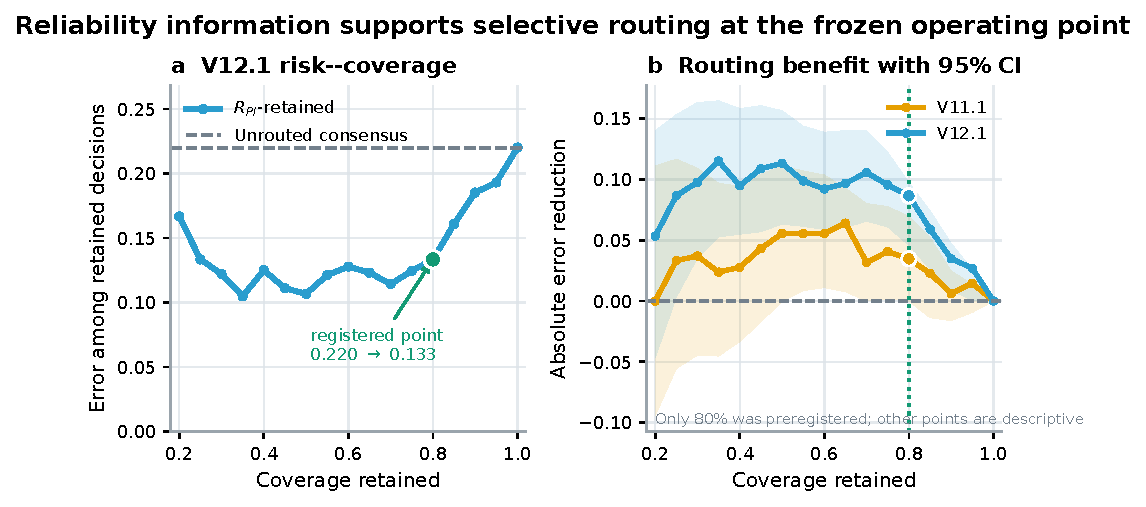
\includegraphics[width=\textwidth]{routing_risk_coverage.pdf}
    \caption{Routing behavior. Left: V12.1 retained error as coverage varies, with the frozen 80\% point highlighted. Right: absolute error reduction and 95\% bootstrap intervals for both held-out runs. Only 80\% coverage was preregistered; all other points are descriptive and are not used for threshold selection.}
    \label{fig:routing}
\end{figure*}

\section{Exploratory Financial Replay}
\label{sec:finance}

The external replay contains 1,247 temporally ordered market rows, an expanding 504-row training window, a five-row label gap, 126-row tests, and six outer folds. Eleven source-specialized statistical agents map to seven provenance roots. Features and calibration use only information visible at decision time. Return statistics are diagnostic only.

\begin{table}[h]
\centering
\small
\begin{tabular}{lrrr}
\toprule
Router & Coverage & Error & AURC \\
\midrule
Confidence & 0.721 & 0.408 & 0.418 \\
AMIR & 0.907 & 0.360 & 0.411 \\
Provenance & 0.709 & 0.359 & 0.431 \\
AMIR no calibration & 0.852 & 0.364 & 0.377 \\
\bottomrule
\end{tabular}
\caption{Exploratory market replay. The favorable AMIR operating point does not establish a significant AURC advantage or prospective financial utility.}
\end{table}

The LLM replay uses the same 500-date manifest in V1 and V2, with 2,500 calls per version. On the 150-date test window, V1's AMIR-style router has coverage 0.920, routed error 0.406, risk Brier 0.240, and risk ECE 0.055, versus majority Brier 0.295 and ECE 0.174. The paired AURC difference is $-0.0874$ with CI $[-0.1994,0.0736]$ in V1 and $+0.0317$ with CI $[-0.0886,0.1805]$ in V2. A prompt-only repair raises valid responses from 68.2\% to 75.6\%; it does not change the non-confirmatory routing verdict.

\end{document}
